	% What kind of text document should we build
	\documentclass[a4,10pt]{article}
	
	
	% Include packages we need for different features (the less, the better)
	
	% Clever cross-referencing
	\usepackage{cleveref}
	
	% Math
	\usepackage{amsmath}
	
	% Algorithms
	\usepackage{algorithm}
	\usepackage{algpseudocode}
	\usepackage{comment}
        \usepackage{url}
	
	% Tikz
	\RequirePackage{tikz}
	\usetikzlibrary{arrows,shapes,calc,through,intersections,decorations.markings,positioning}
	
	\tikzstyle{every picture}+=[remember picture]
	
	\RequirePackage{pgfplots}
	
	
	% Set TITLE, AUTHOR and DATE
        \title{A Project Report on Applied Geometry and Special Effects}
	\author{James Pandey}
	\date{\today}
	 
	
	
	\begin{document}

        % Create the main title section
	  \maketitle
          \begin{center}
            \url{https://github.com/pandeyjames/AppGeoMod}
           \end{center}
          \begin{abstract}
	    This document is a Project Report on the assigned task for STE6247- Applied Geometry and Special Effects.
	
	    This report contains the details of how the task is finalized with added creating the support class for the curves, splines and surfaces to demonstrate how it will exactly can be build in Geometrical Modeling and how their mathematical model can be implemented.
	    The task is done using hardcoded mathematical operations rather than advance option that is already available in GMlib/site GMlib. The functional attributes of curves and B-Spline Curves, and BSpline Surfaces created are integrated and demonstrated, including some basic algorithms and methods.
	
	    The C++ programming language is used to build the application which was provided as a initial setup from Masters of Computer Science study at UiT, Campus Narvik.
	    The application depends on GMlib: Geometric Modeling Library v 0.6.0, and the Qt development suite.
	    The basic features was provided ready-made, with the initial setup and is tasked to implement and build an application which can be used as a template for new applications
	    throughout the MSc computer science study at UiT - Campus Narvik with added functionality and new features.
	  \end{abstract}
	
	
	  %%%%%%%%%%%%%%%%%%%%%%%%%%%%%%%%%%%%%%
	  %%  The main content of the report  %%
	  %%%%%%%%%%%%%%%%%%%%%%%%%%%%%%%%%%%%%%
	 
	
	  \section{Introduction}
            The theoritical background of programming in C++ ~\cite{wesley:2013} is achived during earlier studies.
            Here it is a practical bases of the theories which were studied in the past now has a direct implementation using guide and nomenclature of Qt platform~\cite{guide:2016}
	    The C++ programming language comes with a standard library, the \emph{Standard Template Library} (STL), which consists of containers, methods, algorithms and more.
	
	    Qt (usually pronounced as "cute",) is used mainly for developing application software with graphical user interfaces (GUIs);
	    however, programs without a GUI can be developed, such as command-line tools and consoles for servers.
	    Qt is a cross-platform application framework that is widely used
            for developing application software that can be run on various software and hardware platforms with little or no
            change in the underlying code-base, while still being a native application with the capabilities and speed thereof. Using Qt framework with the Gmlib via GLEW 2.0
            an openGl framework a different approach to Graphic Project is carried out.
	  
            %The demonstration of the output of the program, (see \cref{fig:first_demo}).
	    
            \begin{figure}[ht]
	      \centering
              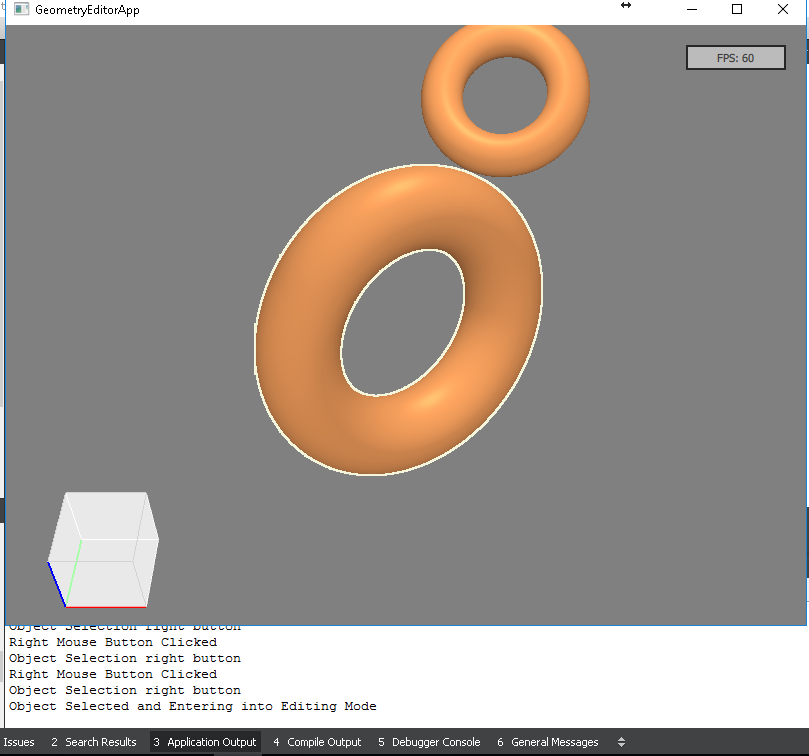
\includegraphics[width=0.8\textwidth]{gfx/first_demo.png}
	      \caption{Demonstration of the Application selection of the object}
	      \label{fig:first_demo}
	    \end{figure}
	
	 
	  \section{Methods}
	    Methods as a way to describe the project includes some various functionality. At the very first default key bind and a simulating Torus object is provided by default in the Application.
	    To develop the application further it is mandatory minimal requirement to bind the keys and mouse events to the default functions for this Qt handles events as signal and slots. 
	    The main idea behind this is to connect the events of keyboard and mouse to the application as QEvent and then the identified events can be used to perform different functions.
	    The mouse and keyboard events such as key presses and button clicked and wheel events are distinguished and then additionally, they are used further to call various methods built in the scenario class
	    as per requirement. Here some functions like selection, deselection, camera movement, object rotation, scale, move, insert and delete can be performed. The main theme of task is to provide
	    manipulation of the objects like a geometrical object such as Torus, sphere, cone, beizier, cylinder, editor, performing the different operations upon.

\newpage
\begin{figure}[h]
              \centering
              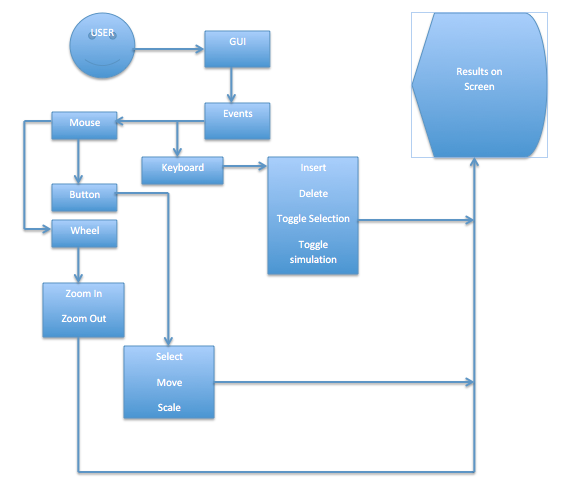
\includegraphics[width=0.9\textwidth]{gfx/flowchart.png}
              \caption{Demonstration the flow of the diagram}
              \label{fig:manipulate}
            \end{figure}
	
	  \section{Discussion}
          As of now the project concludes with the implementations of basic functionality. A head-start with the application is to
          first setup the system which require a graphic card supports openGl version above 4, experienced with version 3 so it is recommended above v 4. If you are a developer and want to further develop the program you need to prepare your system first with Glew v 2.0 and Gmlib v 0.6.0 and of-course have a Qt mingw32 v 5.7 installed.
	For the user of this program only needs to run the supplied released executable file with supported libraries and dll's.
	
	
	As it's an individual project the features which were to be added can't be implemented properly cause one should focus each and every aspect of the project. 
	If it was a group project then more outstanding outcome could be seen, whereas one must only focus on one module and enhance it as the best. 
	This is the main difficulty of the project and lack of references and proper documentation and examples of the implementation of GMlib library was a new thing to approach, 
	which obviously increase the complexity of the task. And limited time frame of only couple of weeks also hardens the way for the accomplishment.
	Some key points of topics for this section:
	    \begin{itemize}
	      \item The application is only developed and tested for windows may not be compatible for other system.
	      \item The version of Glew and the Gmlib pre-match is mandatory otherwise the program may crash with failure.
	      \item Qt framework is a very user friendly with the documentation and help provided online and offline.
	      \item For now the program only runs under windows system future enhancement may include running under other systems.
	      \item A full featured application which can work with the geometrical objects like the software, Auto Cad, Solid work, is
	      an example of the Geometrical Editor. This project may be enhanced with such features in future.
	    \end{itemize}

        \section{Results}
	As we can see the results of the program outcome various output of the application are listed herewith. Every function can't be present out properly here in the report as a pictorial form. So, here some prime functions are included as pictures.
	     
	    A figure below demonstrates a new object sphere insertion in the scene with the main torus deleted. \cref{fig:manipulate}.

\begin{figure}[h]
  \centering
  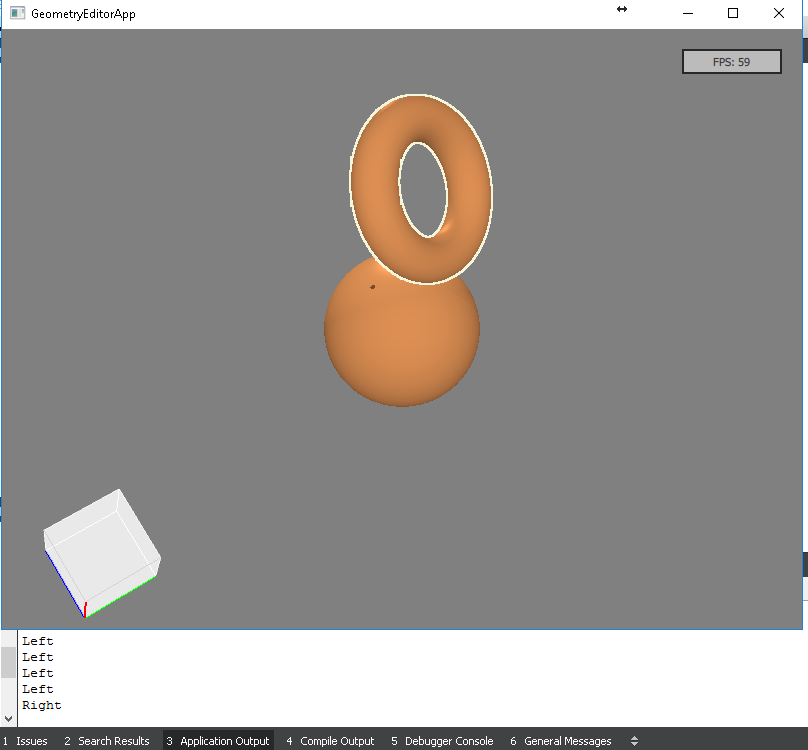
\includegraphics[width=0.65\textwidth]{gfx/manipulate.png}
  \caption{Demonstration of the Application insertion and deletion of the object}
  \label{fig:manipulate}
\end{figure}
\begin{figure}[]
\centering
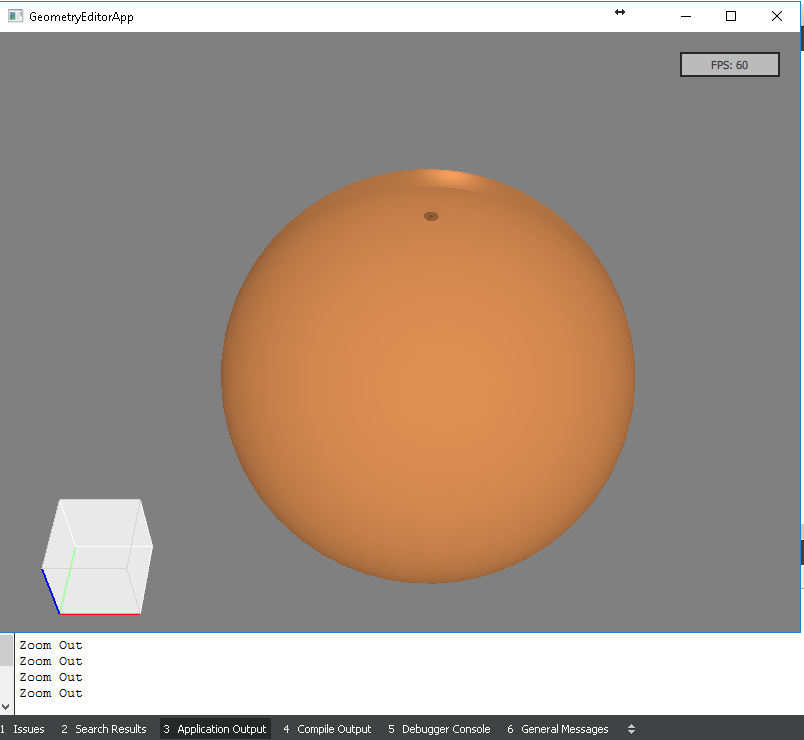
\includegraphics[width=0.45\textwidth]{gfx/zoom.png}
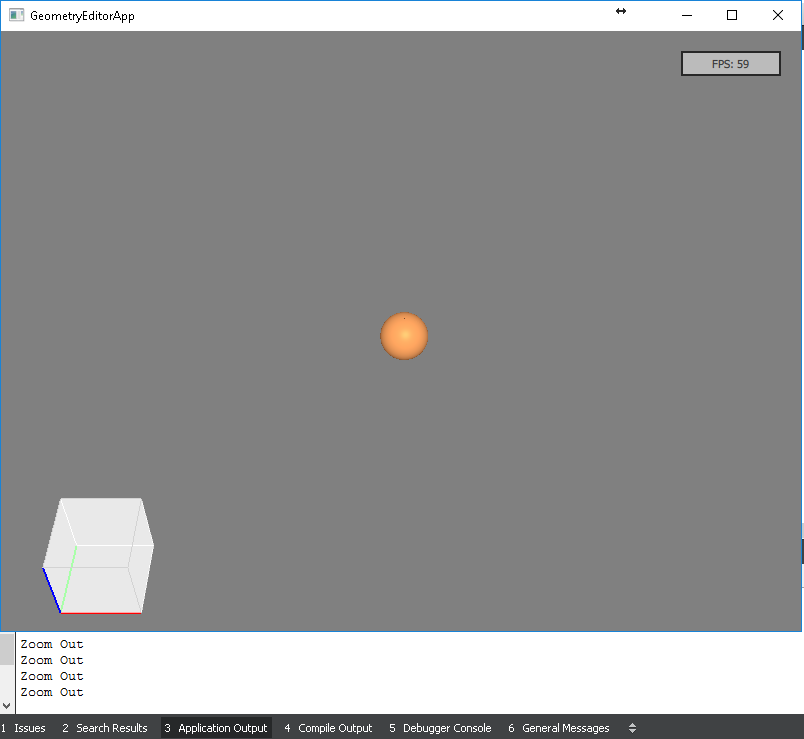
\includegraphics[width=0.45\textwidth]{gfx/zoomout.png}
\caption{Demonstration of the Application zoom in zoom out of object}
\label{fig:zoom}
\centering
\includegraphics[width=0.45\textwidth]{gfx/insertsphere.png}
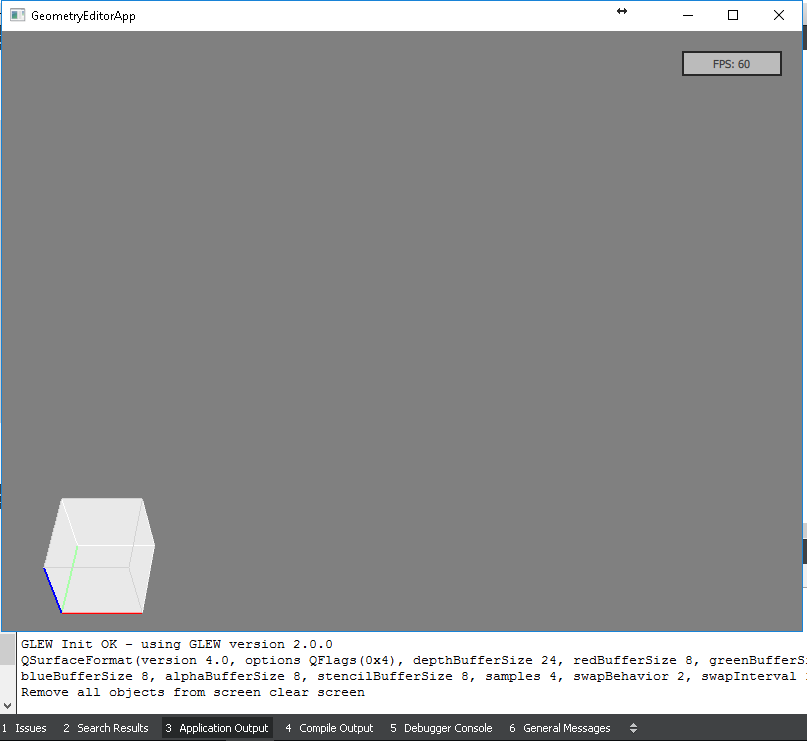
\includegraphics[width=0.45\textwidth]{gfx/clearscreen.png}
\caption{Demonstration of the Application inserting sphere and clearing screen}
\end{figure}
\begin{figure}[]
  \centering
  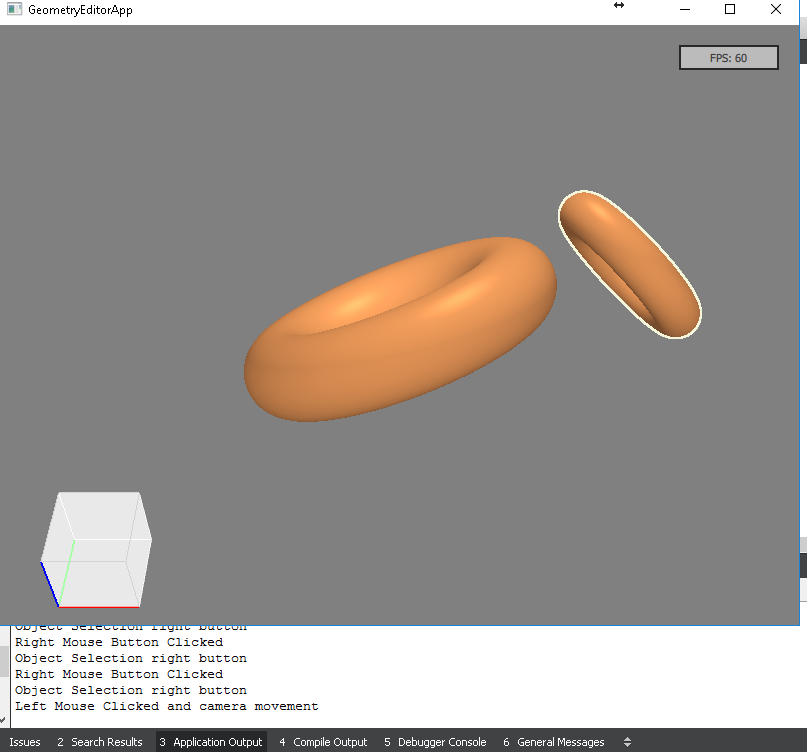
\includegraphics[width=0.45\textwidth]{gfx/rotate1.png}
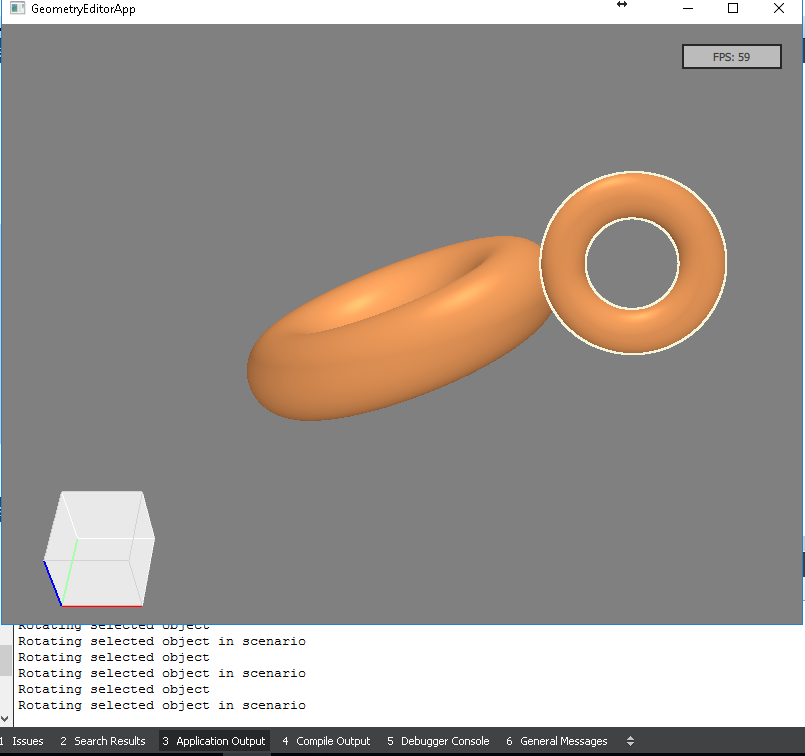
\includegraphics[width=0.45\textwidth]{gfx/rotate2.png}
\caption{Demonstration of the Application zoom in zoom out of object}
\end{figure}
\begin{figure}[]
  \centering
  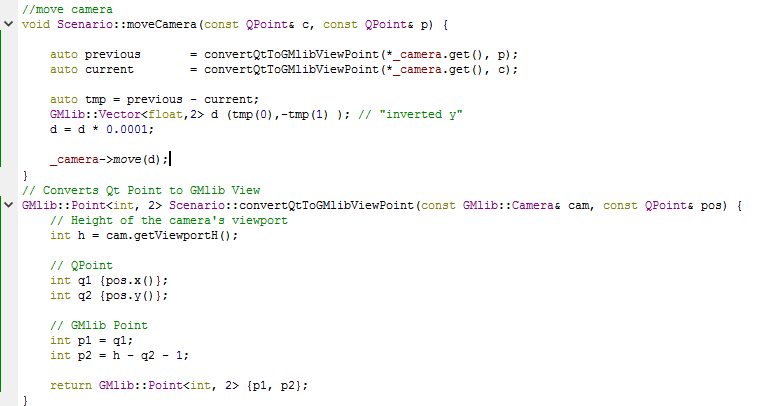
\includegraphics[width=1\textwidth]{gfx/movecamera.png}
  \caption{Codes to handle camera movement}
  \label{fig:movecamera}
\end{figure}
\begin{figure}[]
\centering
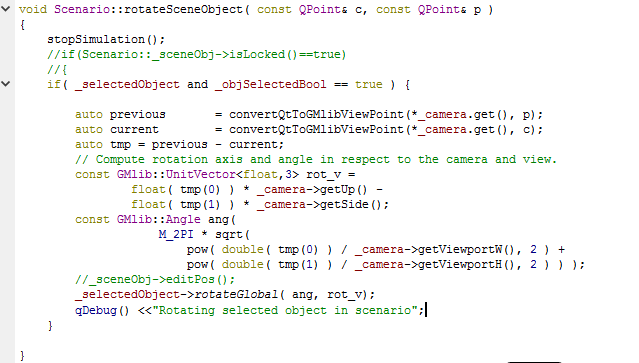
\includegraphics[width=1\textwidth]{gfx/rotateobject.png}
\caption{Codes to rotate scene object}
\label{fig:rotateobject}
\end{figure}
\begin{figure}[]
\centering
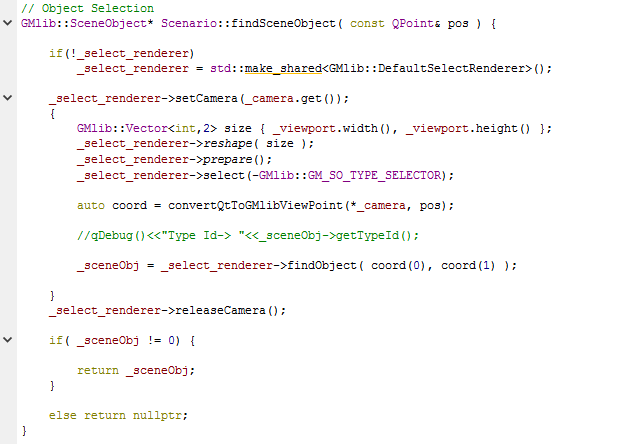
\includegraphics[width=1\textwidth]{gfx/select.png}
\caption{Codes to select object on the screen}
\label{fig:rotateobject}
\end{figure}
\begin{figure}[]
\centering
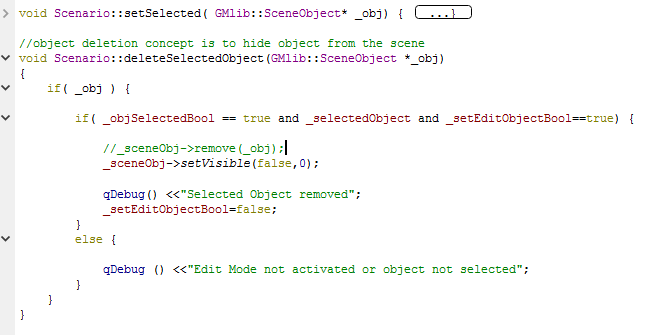
\includegraphics[width=1\textwidth]{gfx/deleteobject.png}
\caption{Codes to delete object on the screen}
\label{fig:rotateobject}
\end{figure}
\pagebreak
\section{Conclusion}
            Future enhancements may include array of object insertsion to the scene manipulation with ease and creating a live object like a car, snowman, with the objects added and various editing functions like scale, resize, delete, insert, with multiple type of object.
            The saving and loading of the scene objects is carried out with openddl data sctucture, where all the properties of the scene objects can be loaded to a structure and can be retrieved afterwards also it is a means of sharing files or objects created by other friends around, but need to use the same structure format.

% Include the bibliography
	  \bibliographystyle{plain}
	  \bibliography{bibliography}
	
	\end{document}
